%%%%%%%%%%%%%%%%%%%%%%%%%%%%%%%%%%%%%%%%%%%%%%%%%%%%%%%%%%%%%%%%%%
%%%%%%%% ICML 2011 EXAMPLE LATEX SUBMISSION FILE %%%%%%%%%%%%%%%%%
%%%%%%%%%%%%%%%%%%%%%%%%%%%%%%%%%%%%%%%%%%%%%%%%%%%%%%%%%%%%%%%%%%

\def\S{K}
\def\reals{\mathbb{R}}
\def\tr{\mathrm{tr}}
\def\cS{\mathcal{S}}
\def\cL{\mathcal{L}}
\def\U{\mathcal{U}}
\def\hp{\hat{p}}
\newtheorem{theorem}{Theorem}

% Use the following line _only_ if you're still using LaTeX 2.09.
%\documentstyle[icml2011,epsf,natbib]{article}
% If you rely on Latex2e packages, like most moden people use this:
\documentclass{article}

% For figures
\usepackage{graphicx} % more modern
%\usepackage{epsfig} % less modern
\usepackage{subfigure}

% For citations
\usepackage{natbib}

% For algorithms
\usepackage{algorithm}
\usepackage{amsfonts}
\usepackage{algorithmic}

% As of 2010, we use the hyperref package to produce hyperlinks in the
% resulting PDF.  If this breaks your system, please commend out the
% following usepackage line and replace \usepackage{icml2011} with
% \usepackage[nohyperref]{icml2011} above.
\usepackage{hyperref}

% Packages hyperref and algorithmic misbehave sometimes.  We can fix
% this with the following command.
\newcommand{\theHalgorithm}{\arabic{algorithm}}

% Employ the following version of the ``usepackage'' statement for
% submitting the draft version of the paper for review.  This will set
% the note in the first column to ``Under review.  Do not distribute.''
\usepackage{icml2011}
% Employ this version of the ``usepackage'' statement after the paper has
% been accepted, when creating the final version.  This will set the
% note in the first column to ``Appearing in''
% \usepackage[accepted]{icml2011}


% The \icmltitle you define below is probably too long as a header.
% Therefore, a short form for the running title is supplied here:
\icmltitlerunning{Actively Learning the Crowd Kernel}

\begin{document}

\twocolumn[
\icmltitle{Capturing the Crowd Kernel}
%or Capturing the Crowd Kernel, Actively?


% It is OKAY to include author information, even for blind
% submissions: the style file will automatically remove it for you
% unless you've provided the [accepted] option to the icml2011
% package.
\icmlauthor{Your Name}{email@yourdomain.edu}
\icmladdress{Your Fantastic Institute,
            314159 Pi St., Palo Alto, CA 94306 USA}
\icmlauthor{Your CoAuthor's Name}{email@coauthordomain.edu}
\icmladdress{Their Fantastic Institute,
            27182 Exp St., Toronto, ON M6H 2T1 CANADA}

% You may provide any keywords that you
% find helpful for describing your paper; these are used to populate
% the "keywords" metadata in the PDF but will not be shown in the document
\icmlkeywords{active learning, crowdsourcing, kernels}

\vskip 0.3in
]

\begin{abstract}
The human notion of perceptual similarity is hard to capture and even more difficult to predict.  Insights into it are invaluable in applications including visual search and GUI design.  In this work we introduce an active Multidimensional Scaling (MDS) algorithm that, given $n$ objects, learns a similarity matrix over all $n^2$ pairs by {\em adaptively} sampling crowdsourced user responses to triplet-based relative similarity queries.  Each query has the form ``is object $a$ more similar to $b$ or to $c$?'' and is chosen to be maximally informative given the preceding responses.  The output is an embedding of the objects into Euclidean space; we refer to this as the ``crowd kernel.''  The runtime (empirically observed to be linear) and cost (about \$0.15 per object) of the algorithm are small enough to permit its application to databases of thousands of objects.  The distance matrix provided by the algorithm allows for the development of an intuitive and powerful sequential, interactive search algorithm which we demonstrate for a variety of visual stimuli.  We present quantitative results that demonstrate the benefit in cost and time of our approach relative to competing approaches, both in the learning stage (quality of estimated distances) and for the end-user at run time (time required to reach goal).  We also show the ability of our approach to capture different aspects of perceptual similarity by demonstrating a variety of binary attribute classifiers (``is striped,'' ``vowel vs.\ consonant,'') trained using the learned kernel.
% comment from Omer: emphasize the end-to-end system in one sentence
\end{abstract}

\section{Introduction}
The problem of capturing and extrapolating a human notion of perceptual similarity has received increasing attention in recent years in domains including vision \cite{Agarwal07}, audition \cite{McFee09}, information retrieval \cite{Schultz03} and a variety of others represented in the UCI Datasets \cite{Xing02,Huang10}.  Concretely, the goal of these approaches is to estimate a similarity matrix $K$ over all pairs of $n$ objects given a (potentially exhaustive) subset of human perceptual measurements on tuples of objects.  In some cases the set of human measurements represents `side information' to computed descriptors (MFCC, SIFT, etc.), while in other cases -- the present work included -- one proceeds exclusively with human reported data, generally obtained via crowdsourcing.  When $K$ is a positive semidefinite matrix induced purely from distributed human measurements, we refer to it as the `crowd kernel' for the set of objects.

Given such a Kernel, one can exploit it for a variety of purposes including exploratory data analysis or embedding visualization (as in Multidimensional Scaling) and relevance-feedback based interactive search.  As discussed in the above works and \cite{Kendall90}, using a {\em triplet based} representation of relative similarity, in which a subject is asked ``is object $a$ more similar to $b$ or to $c$,'' has a number of desirable properties over the classical approach employed in MDS, i.e., asking ``how similar is object $a$ to $b$.''  These advantages include reducing fatigue on human subjects and alleviating the need to reconcile individuals' scales of (dis)similarity.  The obvious drawback with the triplet based method, however, is the potential $O(n^3)$ complexity.  It is therefore expedient to seek methods of obtaining high quality approximations of $K$ from as small a subset of human measurements as possible.  Accordingly, the primary contribution of this paper is an efficient method for estimating $K$ via an information theoretic adaptive sampling approach.  In addition, we contribute an end-to-end system for interactive visual search and demonstrate its benefits -- both quantitative and qualitative -- over competing approaches.


\begin{figure}
\center{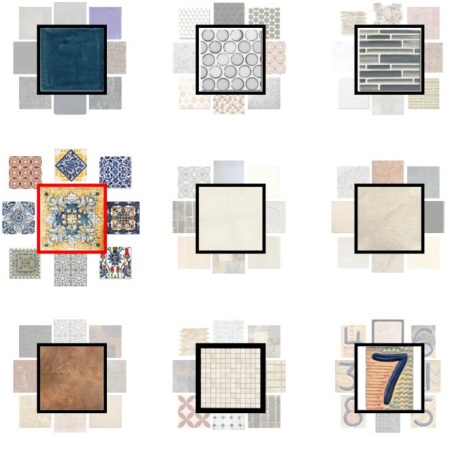
\includegraphics[width=3in]{tiles-tree-top.pdf}} \caption{\label{fig:tilestree} A sample top-level of a similarity search system that enables to a user to search for objects by similarity.  In this case, since the user clicked on the middle-left tile, she will ``zoom-in'' and be presented with similar tiles.}
\end{figure}

\subsection{Findings}
We find that, for a modest price per object, one can capture a Crowd Kernel on general image datasets, across a number of domains.   Active learning helps reduce the costs, or, equivalently, improve performance for a given budget. The Crowd Kernel can be used, among other things, to search for a database of images based on similarity.  Using our system, for example, an online vendor need only input the collection of product images, and the output is a similarity-based browser.  We now describe some general findings about triplet-based similarity measurements using our system on a few different domains, which are somewhat different but in line with previous triplet-based approaches in specific domains.  Then, we describe how our active learning algorithm improves performance.

First, triplet-based questions may seem ill-posed in many domains.  Consider even English letters.  Can people meaningfully answer the question: is the letter `a' more similar to `b' or `c'?  Our experiments show statistically significant consistency with agreement 58\% ($pm$2\%, with 95\% confidence) agreement between users on a random triple.  Greater agreement is observed for random image triplets from an online tie store (68\%) and floor tile images (65\%).  From such triplets, we approximate the crowd kernel by a PSD matrix.  Our kernel predicts future results on such triplets with accuracy ?? on English letters, ?? on tie store images, and ?? on floor tile images.  Second, by learning an SVM with such a kernel, the kernel is shown to contain useful information about human notions of similarity.  For example, for images of the 26 English letters, it perfectly represents the distinction between vowels and consonants and between ``short'' letters, acemnorsuvwxz, and tall ones, bfhkl.  The former is an example of a feature that would be difficult to learn directly from existing computer vision algorithms based upon pixel-level or higher-level (e.g., SIFT) features.  On many domains, it seems feasible for existing computer vision algorithms to represent many important high-level features, e.g., detecting gender from a face image or detecting whether or not a tie is striped, but doing so involves a certain amount of expertise and domain specific tuning.  Hence, approximating the CK alone (without even examining the images) is shown to be useful because, (a) it is not prohibitively expensive for certain domains, such as products (b) it has the potential to learn high-level context-aware features that go beyond the limits of most computer vision/AI systems, and (c) it is practical in that it can be acquired in a uniform fashion across domains without requiring domain-specific expertise.

Finally, the main finding is that active learning does indeed reduce the label complexity in capturing the Crowd Kernel.  Our algorithm has two components: a fitting algorithm which fits a probabilistic model to a sequence of triples, and a selection algorithm that uses the fit to determine which triples to label.  One interesting result here is that an algorithm which fits the data well may nonetheless yield poor suggestions of which triples to label.  Our final loss is nonconvex, but we give algorithms that provably optimize the loss nonetheless.???(I hope!)

The remainder of this paper is organized as follows.  In Section ... blah blah ... (executive summary of remaining sections so reader knows what to expect in each part).


\section{Preliminaries}\label{sec:prelim}

The set of $n$ objects is denoted by $[n]=\{1,2,\ldots,n\}$.  For $a,b,c \in [n]$, a comparison or {\em triple} of the form, ``is $a$ more similar to $b$ or to $c$,'' is denoted by $^a_{bc}$. We write $p^a_{bc}$ for the probability that a {\em random} crowd member rates $a$ as more similar to $b$, so $p^a_{bc}+p^a_{cb}=1$.
The $n$ objects are assumed to have $d$-dimensional Euclidean representation, and hence the data can be viewed as a matrix $M \in \reals^{n \times d}$, and the {\em similarity matrix} $\S \in \reals^{n \times n}$ is defined by $\S_{ab}=M_a\cdot M_b$, or equivalently $\S = MM'$.  Note that $\S$ is necessarily positive semidefinite (PSD), and for any PSD matrix $\S$, one can efficiently find an embedding in $\reals^d$ (unique up to change of basis), for some $d \leq n$.  Also equivalent is the representation in terms of distances, $d^2(a,b)=\S_{aa}-2\S_{ab}+\S_{bb}$.

In our setting, an {\em MDS algorithm} takes as input $m$ comparisons $(^{a_1}_{b_1c_1},y_1) \ldots (^{a_m}_{b_mc_m},y_m)$ on $n$ items, where $y_i\in \{0,1\}$ indicates whether $a_i$ is more like $b_i$ than $c_i$.  Unless explicitly stated, we will often omit $y_i$ and assume that the $b_i$ and $c_i$ have been permuted, if necessary, so that $a_i$ was rated as more similar to $b_i$ than $c_i$.  The MDS algorithm outputs an embedding $M \in \reals^{n \times d}$ for some $d \geq 1.$  A probabilistic MDS model outputs predicts $\hat{p}^{a}_{bc}$ based on $M_a$, $M_b$, and $M_c$.  Our probabilistic MDS models minimize empirical log loss, $\min \sum_i \log 1/\hat{p}^{a_i}_{b_ic_i}$, subject to some regularization constraint.

An {\em active} MDS algorithm chooses each triple, $^{a_i}_{b_ic_i}$, adaptively based on $(^{a_1}_{b_1c_1},y_1) \ldots (^{a_{i-1}}_{b_{i-1}c_{i-1}},y_{i-1})$.
In terms of notation, $M'$ denotes the transpose of matrix $M$, $\|M\|_F=\sqrt{\sum_{ij} M_{ij}^2}$ denotes the Frobenius norm.

\subsection{Why adaptation may help}
We first give high-level intuition for why adaptation may help compared to random queries.  First consider data that naturally partitions into $k \ll n$ disjoint equal-sized clusters, such that between clusters objects are completely dissimilar but within clusters they have varied similarities.  For example, our images from an online tie store, including ties, tie clips, and scarves roughly cluster nicely (though the clusters are very imbalanced).  Say that, knowing which class an object belongs to, one can locate the object using $q$ queries by comparing it to other objects in the same class.  On the other hand, suppose comparisons with objects in two different classes simply yield 50/50 random results if the three objects are in different classes but that the user will select an object of the same class if one exists in the comparison pair.  The number of adaptive queries to learn in such a setting is $\Theta(nk+nq)$ -- $\Theta(k)$ comparisons are required to determine which class each object is in (with high probability) and then an additional $q$ queries are required.  With random queries, one would require $\Theta(n k^2 q)$ queries, because only a $1/k^2$ fraction of the random queries will count towards the $q$ necessary queries within objects of the same class.


Next, consider data representing an underlying rooted tree with $L \ll n$ leaves, inspired by, say, phylogenic trees involving animal species.\footnote{This example is based upon a tree metric rather than a Euclidean one.  However, note that any tree with $L$ leaves can be embedded in $L$-dimensional Euclidean space so that the squared distance between any pair of embedded points is equal to the number of edges in their shortest path on the tree.  Moreover, the rich study of Embeddings (see, e.g., \citealp{IM04}) has shown that many types of metrics can be embedded (to varying degrees of approximation) within Euclidean space.}  Say the similarity between objects is decreasing in their distance in the tree graph and, furthermore, that objects are drawn uniformly at random from the classes represented by the leaves of the tree.  Ignoring the details of how one would identify that two objects are in the same leaf or subtree, it is clear that a nonadaptive method would have to ask $\Omega(n L)$ questions to determine the leaves to which $n$ objects belong (or at least to determine which objects are in the same tree).  On the other hand, in an ideal setting, an adaptive approach might determine such matters using $O(n \log L)$ queries in a balanced binary tree, assuming a constant number of comparisons can determine to which subtree of a node an object belongs, hence an exponential savings.

\section{Previous work}

TO ADD!

\section{Our algorithm}

Our algorithm proceeds in phases.  In the first phase, it queries a certain number of random triples comparing each object $a \in [n]$ to random pairs of distinct $b,c$.  (Note that we never perform a triple where $a=b$ or $a=c$ except for quality control purposes.) Subsequently, if fits the results to a matrix $M \in \reals^{n \times d}$ using the ``relative'' probabilistic model described below.  Then it uses our adaptive selection algorithm to select further random triples.  This iterates: in each iteration all previous data is fit to the relative MDS model, and then the adaptive selection algorithm generates more triples.  We first describe the probabilistic MDS model, starting with a natural logistic model first and then addressing its shortcomings with the relative model.  We then describe our adaptive selection procedure.  Further details and system parameters are given in Section \ref{sec:parameters}.

\subsection{Probabilistic models}

[Add related work about probabilistic MDS models if there is any, mention max-margin models]

Initially, a random set of triples is drawn.  Then, iteratively, triples are added to compare each item to others.  We first describe the probabilistic models and how to fit them to arbitrary labeled triples, without specifying how the triples are selected.

The first model is based upon logistic regression, and hence we refer to it as the `logistic model.'  This model aims to find a matrix $\S$ so that,
\begin{equation}\label{eq:logistic}
\hat{p}^a_{bc} = \frac{e^{\S_{ab}}}{e^{\S_{ab}}+e^{\S_{ac}}} = \frac{1}{1+e^{\S_{ac}-\S_{ab}}}.
\end{equation}
Note that $\log 1+e^{\S_{ac}-\S_{ab}}$ is a convex function of $\S\in \reals^{n\times n}$.  Hence, for any convex set $W \subseteq \reals^{n \times n}$, the problem of minimizing empirical log loss, $\cL(\S)=\min_{\S \in W} \sum_i \log 1/\hp^{a_i}_{b_ic_i}$, is a convex optimization problem.  Now, requiring $\S \succeq 0$ is not very restrictive since any $\S+kI \succeq 0$ for large enough $k>0$, i.e., by a sufficiently large increase in the diagonal, any symmetric matrix becomes PSD. This means that generalization would require $\Omega(n^2)$ data.  Hence, in addition to requiring $\S \succeq 0$, we consider three natural regularization constraints.  The first is a {\em rank} regularization, simply to bounding to be at most some $d\ll n$, which can be done effectively by forcing an embedding $M \in \reals^{n \times d}$.  One can perform gradient descent directly on $\cL(MM')$, though this may get trapped in local minima since the loss function is not convex in $M$.  The second approach would be a {\em trace} constraint bounding $\sum_i \S_{ii}$ below a specified value. The third regularization is a {\em diagonal constraint} asserting that $\S_{11}=\S_{22}=\ldots=S_{nn}$ are all some fixed value.  For the latter two cases, these are convex optimization problems which may be solved with the {\em gradient projection method}, in which one computes a sequence of approximations, $\S^0=\lambda I$ and $\S^{t+1}= \Pi_W(S^t - \eta \nabla \cL(S))$ where, for set $W \subseteq \reals^{n \times n}$, $\Pi_W(S)=\arg\min_{T \in W} \|\S-T\|_F^2$ is the closest matrix in $W$ to $S$.  Note that both $\{\S \succeq 0~|~\tr(S)\leq nr\}$ and $\{\S \succeq 0~|~\S_{ii}=r\}$ are convex sets for any $r\geq 0$.  Projection to the closest trace-bounded PSD matrix involves a single SVD along with soft thresholding.  Projection to the closest PSD matrix with a fixed diagonal is discussed in Section \ref{sec:proj}, and is closely related to recent work on the max-norm of matrices \cite{SS05,??}.

As discussed in Section \ref{sec:logisticexp}, fitting the logistic model fits data well and reproduces interesting features, such as vowel/consonant or stripedness.  However, empirically it performs poorly in terms of deciding which triples to ask.  Figure \ref{fig:exp} gives a simple example illustrating where the exponential model chooses a poor question.  To see why, note that $p^{b}_{bc}=\frac{1}{1+exp(b\cdot(c-b))}$ and $p^{c}_{bc}$ are both very close to $1/2$ because $b\cdot (c-b)$ and $c \cdot (b-c)$ are both close to 0.  This, in itself, is somewhat strange because one would definitely expect that $b$ should be generally be predicted to be much more similar to $b$ than to $c$.  On the other other hand, $p^{b}_{uv}=1-p^{c}_{uv} \gg 1/2$ since $b\cdot (x-y)=-c \cdot (x-y)\gg 0$.

\begin{figure}
\center{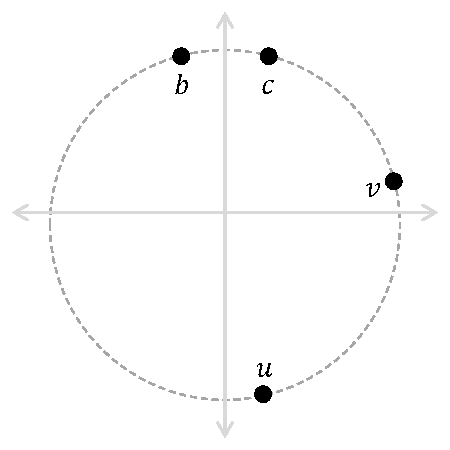
\includegraphics[width=3in]{expfig.pdf}} \caption{\label{fig:exp} When unsure whether a point is at location $b$ or $c$, the logistic model would strangely prefer comparing it to $u$ \& $v$ over $b$ \& $c$.}
\end{figure}

This criterion for evaluating a model, namely what quality triples it suggests asking, is an interesting one.  The second model addresses this problem, and is motivated by the scale-invariance observed in many perceptual systems (see, e.g., \citealp{CB99}).  Let $\delta_{ab} = \|M_a-M_b\|^2=S_{aa}+S_{bb}-S_{ab}$.  A very simple scale-invariant model takes $\hat{p}^a_{bc} = \frac{\delta_{ac}}{\delta_{ab}+\delta_{ac}}$.  According to such a relative model (termed relative because it relates to ratios), if one was unsure whether a point was at $b$ or $c$, comparing it to $b$ and $c$ would give a perfect indication of where it is.  Again even for $S$, such a model must also be regularized or else it would have $\Theta(n^2)$ degrees of freedom.  Here again, one may regularize by the rank of $S$, the trace or bounding $\S_{ii}$.  Due to the scale-invariance of the model, however, even these constraints do not have enough bite.  In particular, note that halving or doubling the matrix $M$ doesn't change any probabilities.  Hence, descent algorithms may lead to very small, large, or numerically unstable solutions.  To address this, we modify the model as follows, for distinct $a,b,c$:
\begin{equation}
\label{eq:rel}
\hat{p}^a_{bc} =  \frac{1+\delta_{ac}}{2+\delta_{ab}+\delta_{ac}} \mathrm{ and } \S_{ii}=r,
\end{equation}
for some parameter $r>0$.  In fact, this is really more of an additional assumption than a modification -- the above is equivalent to the $\frac{\delta_{ac}}{\delta_{ab}+\delta_{ac}}$ where we suppose each object as having a minimal amount of ``uniqueness,'' $\mu>0$, which means $\S = \mu I + T$, where $T \succeq 0$. For the moment, also fix $T_{ii}=1$ and hence $\S_{ii}=1+\mu$.  This is equivalent to each object having a separate coordinate in which it is at least $\sqrt{\mu}$ and every other object is 0.  In this case, the model reduces to,
\begin{eqnarray*}
\hat{p}^a_{bc} &=& \frac{2\mu + T_{aa}+T_{cc}-2T_{ac}}{4\mu+2T_{aa}+T_{cc}+T_{bb}-2T_{ab}-2T{ac}}\\
&=&\frac{1 + \frac{1}{2\mu}(T_{aa}+T_{cc}-2T_{ac})}{2 + \frac{1}{2\mu}(2T_{aa}+T_{cc}+T_{bb}-2T_{ac}-2T_{ab})}.
\end{eqnarray*}
Finally, substituting $\S$ for $\frac{1}{2\mu}T$ and $r=\frac{1}{2\mu}$ gives exactly the model in (\ref{eq:rel}).  Again, the model can be fit in low-dimension by doing gradient descent directly on $M$ or in high dimensions using the gradient projection method on $\S$.  Here $\mu$ serves the same purpose as a margin constraint and the fixed constant 1 is analogous to fixing the margin to 1 and upper bounding the length of vectors to $r$. 

This model is appealing in that it fits the data well, suggests good triples, and also represents interesting features on the data.  Unfortunately, the model itself is not convex.  Interestingly, we are able to prove that error of the algorithm will be optimal, by showing that gradient descent will converge to the ``true'' $S^*$ if there is one.
\begin{theorem}
To add.
\end{theorem}


\section{Adaptive selection algorithm}

We describe the adaptive selection algorithm with respect to the relative model above, but it can equally well be applied to the exponential model.  The idea is to capture the uncertainty about the location of an object through a probability distribution over points in $\reals^d$, and then to ask the question that maximizes information gain.  More precisely, say we are given an embedding of $n$ objects represented by matrix $M$ (or $S$), along with comparisons.  For each object $a=1,2,\ldots,n$, we generate a new triple to compare $a$ to, as follows.  Say users have previously rated $a$ as more similar to $b_i$ than $c_i$, for $i=1,2,\ldots,j-1$, and we want to generate the $j$th query, $b_j,c_j$ (this is a slight abuse of notation because we don't know which of $b_j$ or $c_j$ will be rated as closer to $a$).  We also require a prior distribution $\pi$ over $\reals^n$, to be described shortly.  The observations imply a posterior distribution of $\rho(x) \propto \pi(x) \prod_i \hp^{x}{b_ic_i}$ over $x \in \reals^d$.  This distribution captures the uncertainty.  Given any candidate query for objects in the database $b$ and $c$, the model predicts that a user will rate $a$ as more similar to $b$ than $c$ with probability $p=\sum_x \rho(x)\frac{\delta(x,c)}{\delta(x,b)+\delta(x,c)}$.\footnote{Like other active learning models, e.g. \cite{??}, it is tempting to choose $b$ and $c$ so as to make this probability close to $1/2$.  In our case, this is not sufficient because $b$ and $c$ could be known to give $p$ close to half without being a useful query, e.g., $b$ and $c$ are very close to one another but far from $a$.  However, we wouldn't want to compare $a$ to $b$ and $c$ repeatedly in this case.}  If it rates $a$ more similar to $b$ than $c$ it has a posterior distribution of $\rho_b(x) \propto \rho(x)\frac{\delta(x,c)}{\delta(x,b)+\delta(x,c)}$ and there is a similarly-defined posterior distribution if $a$ were rated as more similar to $c$ than $b$.  The {\em information gain} of this query is defined to be $H(\rho)-pH(\rho_b)-(1-p)H(\rho_a)$, where $H(\rho)$ gives the entropy of probability distribution $\rho$.  The algorithm greedily selects a query, among all pairs $b,c \neq a$, which maximizes information gain.  This computation can be a bit slow (seconds per object in our datasets), so for efficiency we take the best pair from a selection of 500? random pairs.  

It remains to explain how we generate the prior $\pi$.  We take $\pi$ to be the uniform distribution over the set of points in $M$.  Hence, the process can be viewed as follows.  For the purpose of generating a new triple, we pretend the coordinates of all other objects are perfectly known, and we pretend that the object in question, $a$, is an unknown one of these other objects.  The chosen pair is designed to maximize the information we receive about which object it is, given the observations we already have about $a$.  The hope is that, for sufficiently large data sets, such a data-driven prior is a reasonable approximation to the actual distribution over data.  This approach worked in our experiments, but it does seem to be limited to achieving accuracy related to the nearest neighbor in the dataset.  Another natural alternative prior would be a multinormal distribution fit to the data in $M$.





\section{Experiments and Applications}

%4a. floor tiles and/or flags
%first part: learning the human kernel for this
%- example triplets: what mturkers saw, also show how triplets change with adaptivity (vs. random)
%- embedding: projected into 2D (possibly snapped to grid)
%- nearest neighbor examples (when it's done training)
%- attribute discovery: user takes set of embedded "feature vectors," sets up supervised learning problem by labeling subset of training examples that have a %certain attribute (e.g., zig zag pattern), trains SVM to extrapolate to remaining examples; this shows the descriptive power of the embedded representation
%- quantitative plots: triplet preference prediction accuracy vs. time/money invested into crowdsourcing for different adaptive sampling methods and different %fitting methods
%- observed training/run time
%second part: using the human kernel to build a visual search interface
%- describe interactive/sequential search interface with blocks of 9 choices user can click
%- question is: how long/how many clicks does it take to get to desired object
%-- user may expect clustery feel; we need to emphasize that what we're shooting for is smallest number of clicks to get to desired target
%- performance evaluation: number of clicks averaged over many object instances, prediction accuracy for which of the 9 images they click on
%4b-d. more example domains
%- letters a-z?

We experiment on four datasets: (1) images of twenty-six lowercase letters, (2) 223 flag images, (3) 433 tile images from Amazon, and (4) 300 product images from an online tie store.  We find that, for certain ranges of parameters, adaptive queries can achieve the same performance as uniformly random queries using roughly half of the queries, or equivalently, for half of the cost.  There are many ideas for how one might improve the system and we hope that further work will show dramatic gains.

For ease of implementation, we assume all users are identical.  This is a natural starting point, especially given that our main focus is on active learning.

Figure \ref{fig:adaptive-trips} illustrates the adaptive triples selected on the tiles dataset, along with the answers given by users.
\begin{figure}
\center{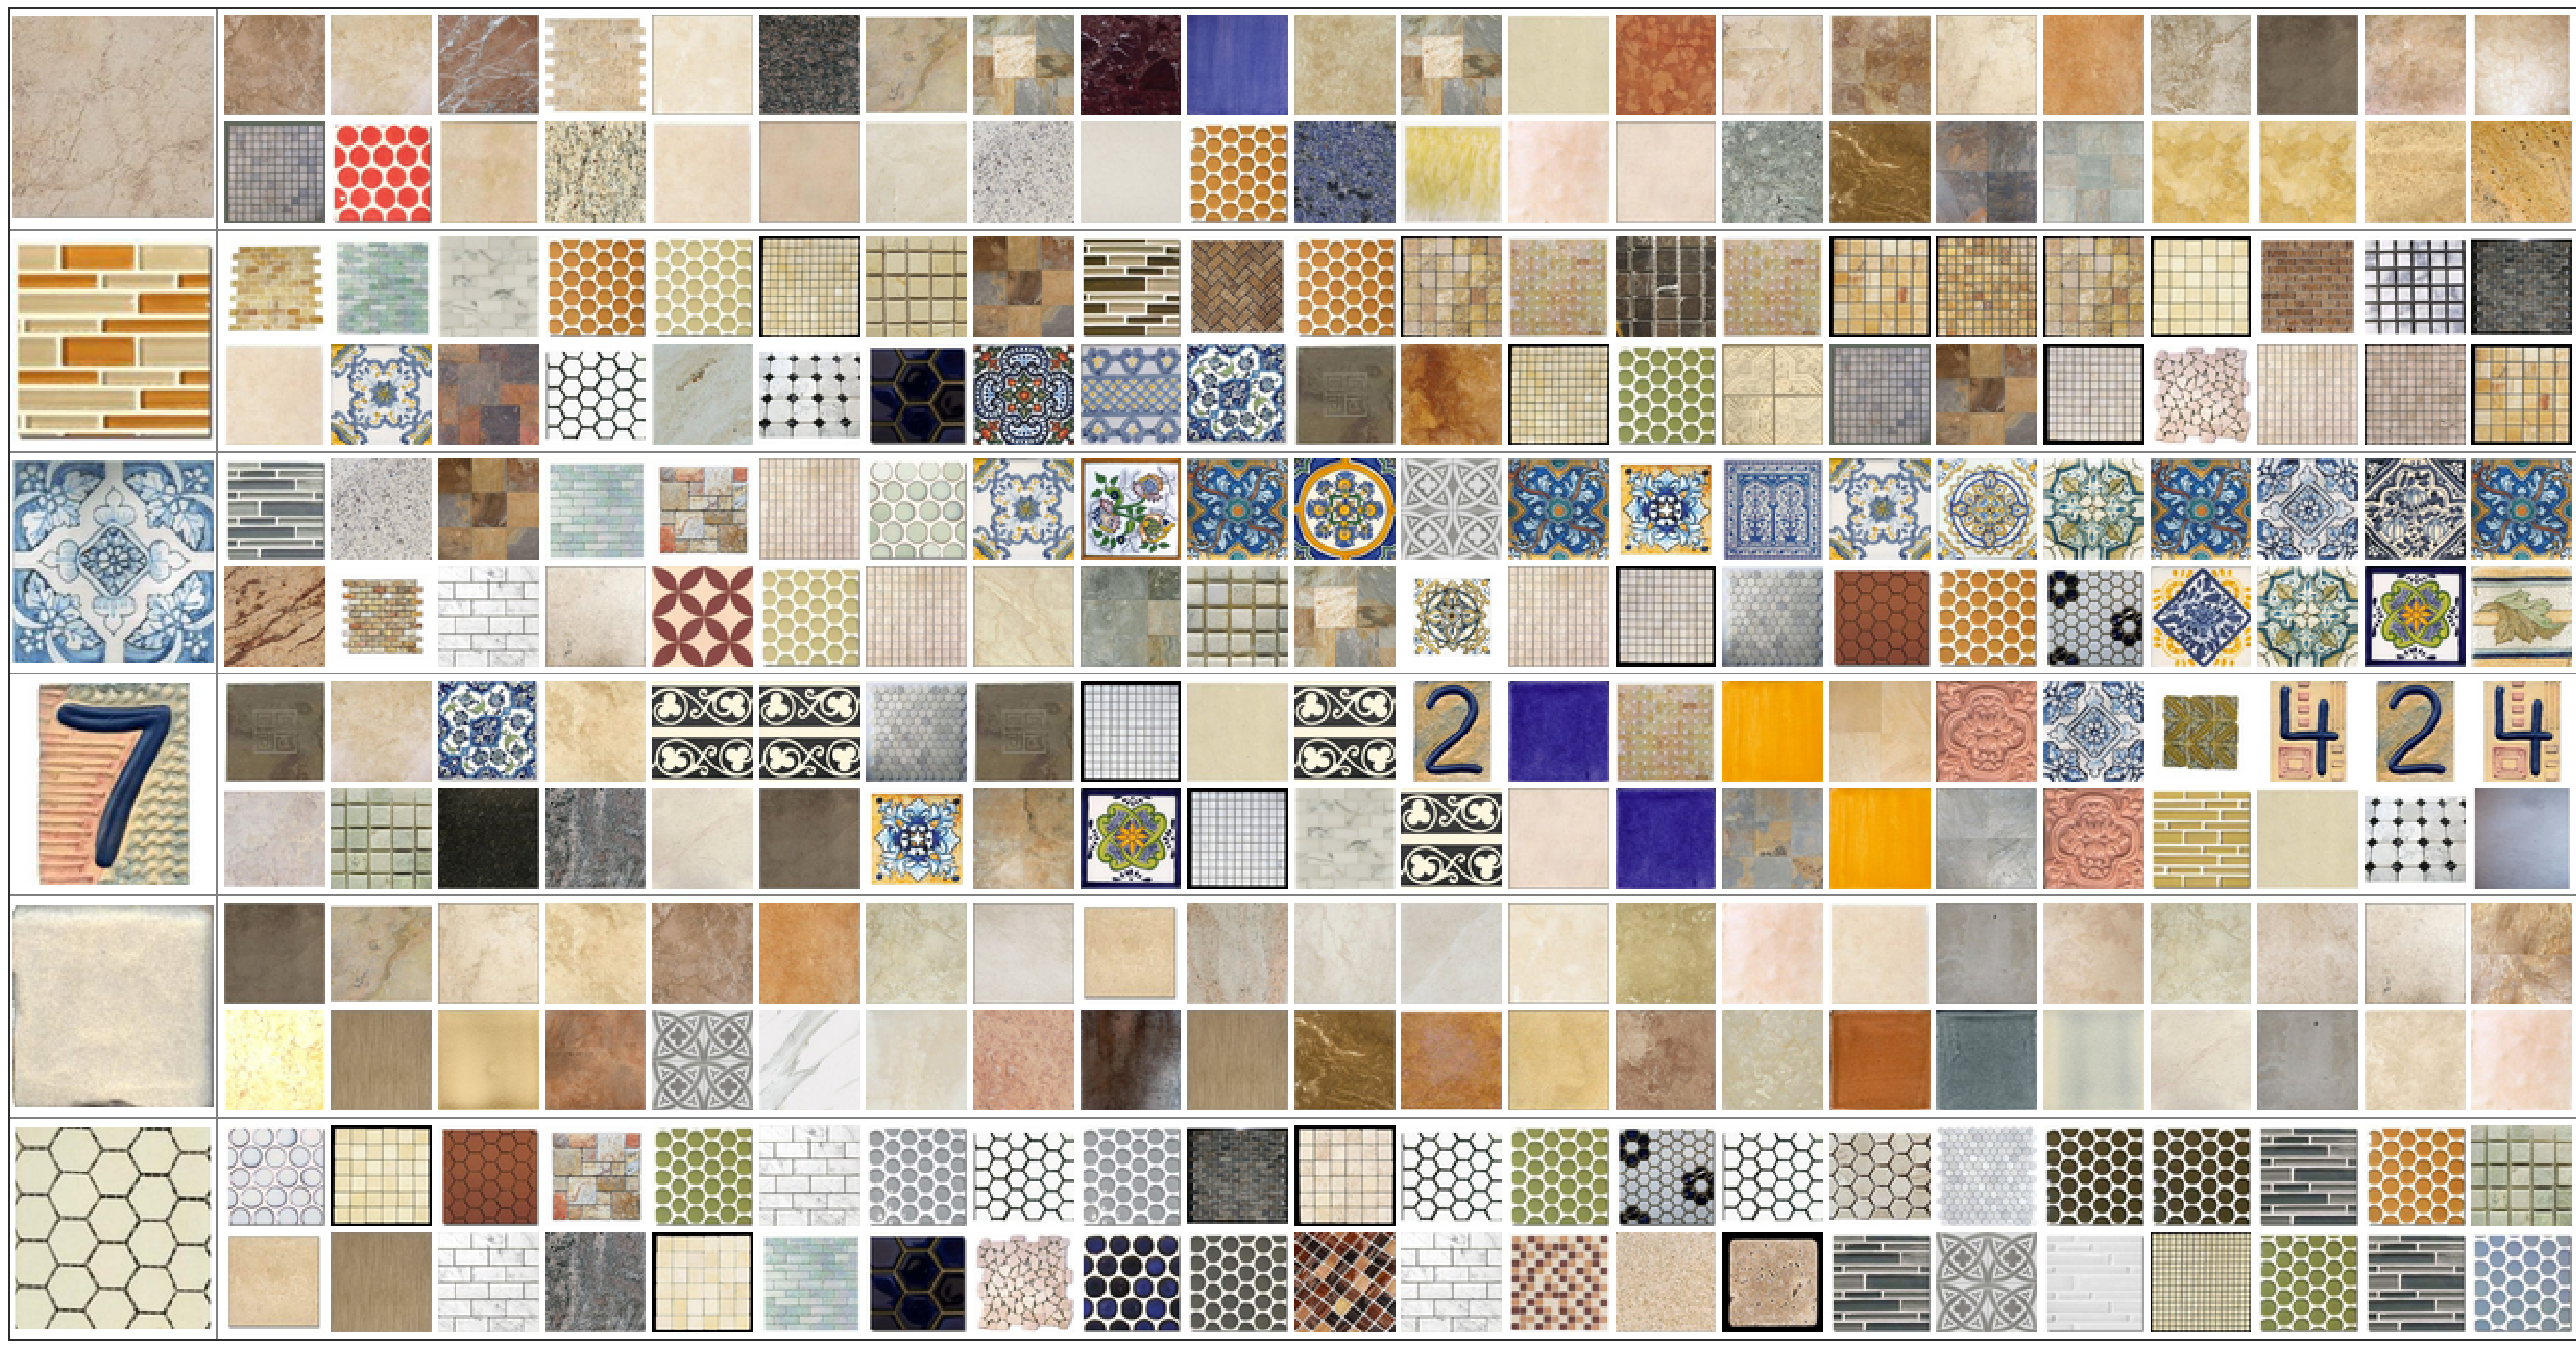
\includegraphics[angle=270,width=3in]{tiles_adaptive.pdf}} \caption{\label{fig:adaptive-trips} A sample top-level of a similarity search system that enables to a user to search for objects by similarity.  In this case, since the user clicked on the middle-left tile, she will ``zoom-in'' and be presented with similar tiles.}
\end{figure}


\subsection{20Q Metric}
It is not clear how to judge the predictions that a particular embedding implies.  One application of such systems is search, i.e., searching for an item that a user knows what it looks like (we assume that the user can answer queries as if she even knows what the store image looks like).  Therefore, it is natural to ask how well we have ``honed in'' on the desired object after a certain number of questions.  For our metric, we suppose that the user has selected a secret random object in the database and the system is allowed to make query 20 triples, adaptively (as in the game ``20 questions''), after which it produces a ranking of items in the database.  The metric is the average position of the random target item in this list.  This metric is meant to roughly capture performance, but of course in a real system users may not have the patience to click on twenty pairs of images and may prefer to choose from larger sets. (Our system has the user select one of 8 or 9 images, which could potentially convey the same information as 3 binary choices.)  

\subsection{Using the Kernel to classify}

The learned Kernels may be used in a linear classifier such as a support vector machine.  This helps elucidate which features were used by humans in labeling the data.  In the experiments below, images were labeled with binary $\pm$ classes and ? indicating don't care.  For example, if the classification task is identifying whether a tie is striped or not, labeling the tie clips seems irrelevant and we ignore them.  The LIBSVM \cite{CC01} package was used with default parameters.  For all learning tasks but letters, results are shown on 30? held-out examples while the rest were used for training.  For the letters, we show results based on leave-one-out classification.  The results are shown by sorting the held-out images form left to right in order of their inner product with the learned direction.  In addition, the following table summarizes accuracy on a variety of tasks.

\subsection{Nearest neighbors and PCA}
Below we show the nearest neighbors for the tiles and flags data sets.

{\center 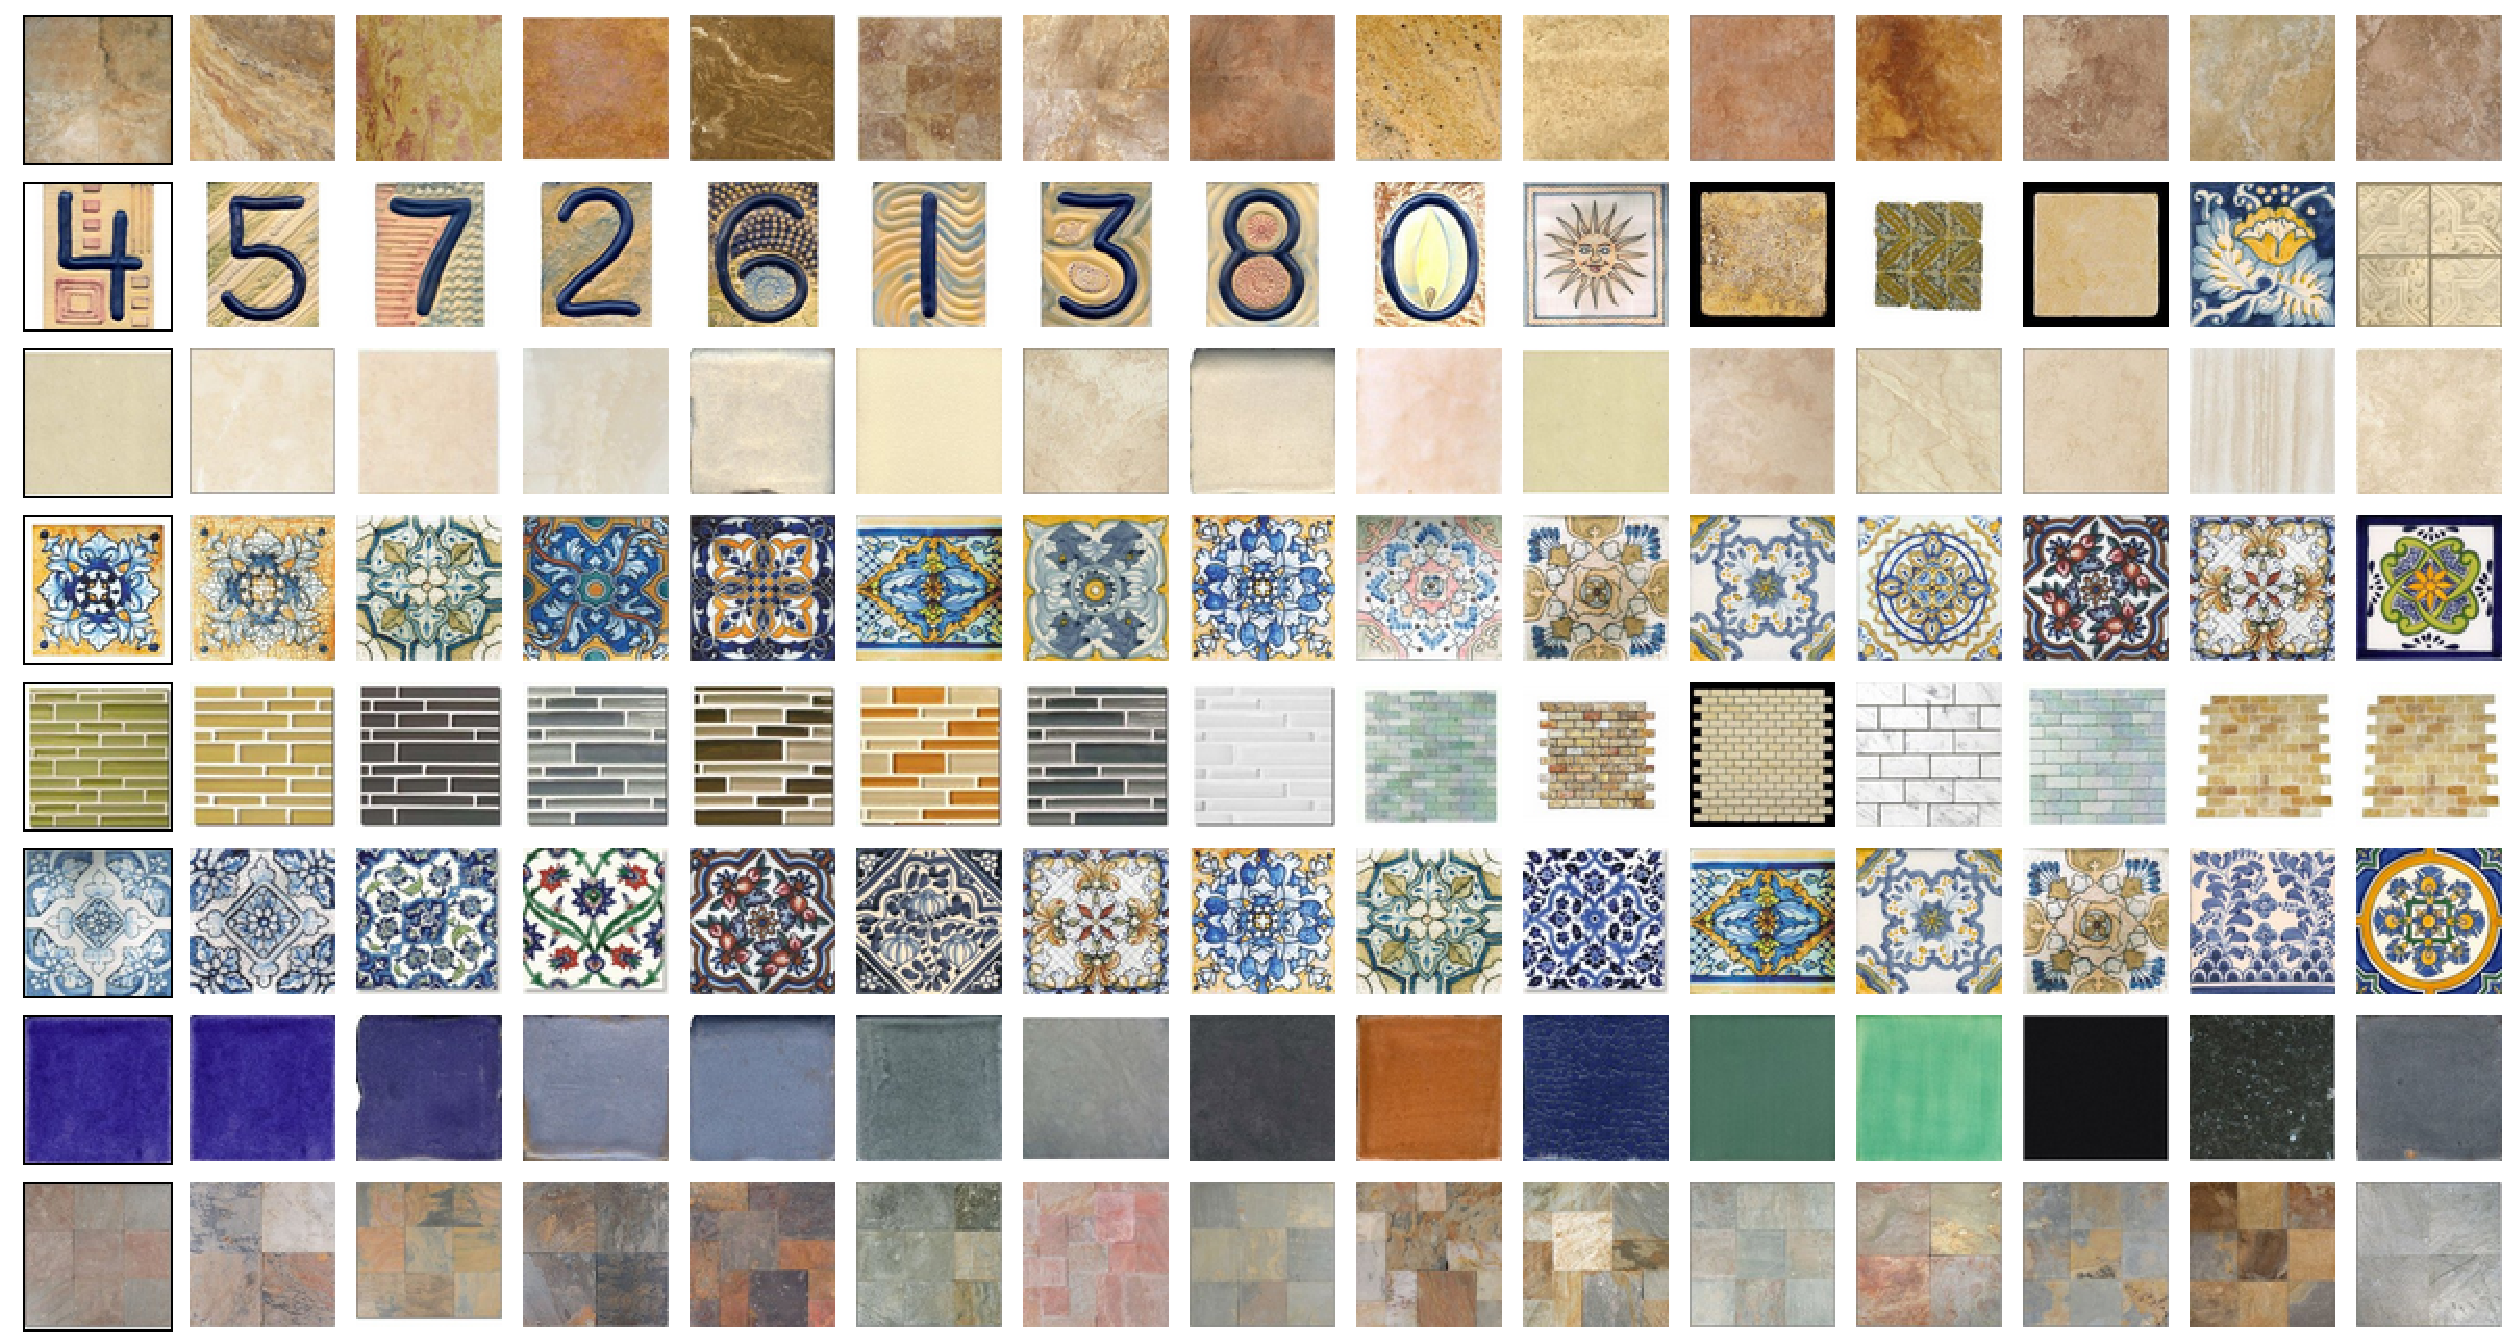
\includegraphics[width=3.5in]{tiles_neighs.pdf}} 

The reference image is on the left and the 14 nearest neighbors are displayed from left to right.

{\center 
\includegraphics[width=3.5in]{flags_neighs.pdf}}

Below, the tie store images are displayed according to their projection on the top two principal components of a PCA.  (The principal component is the horizontal axis.)
{\center 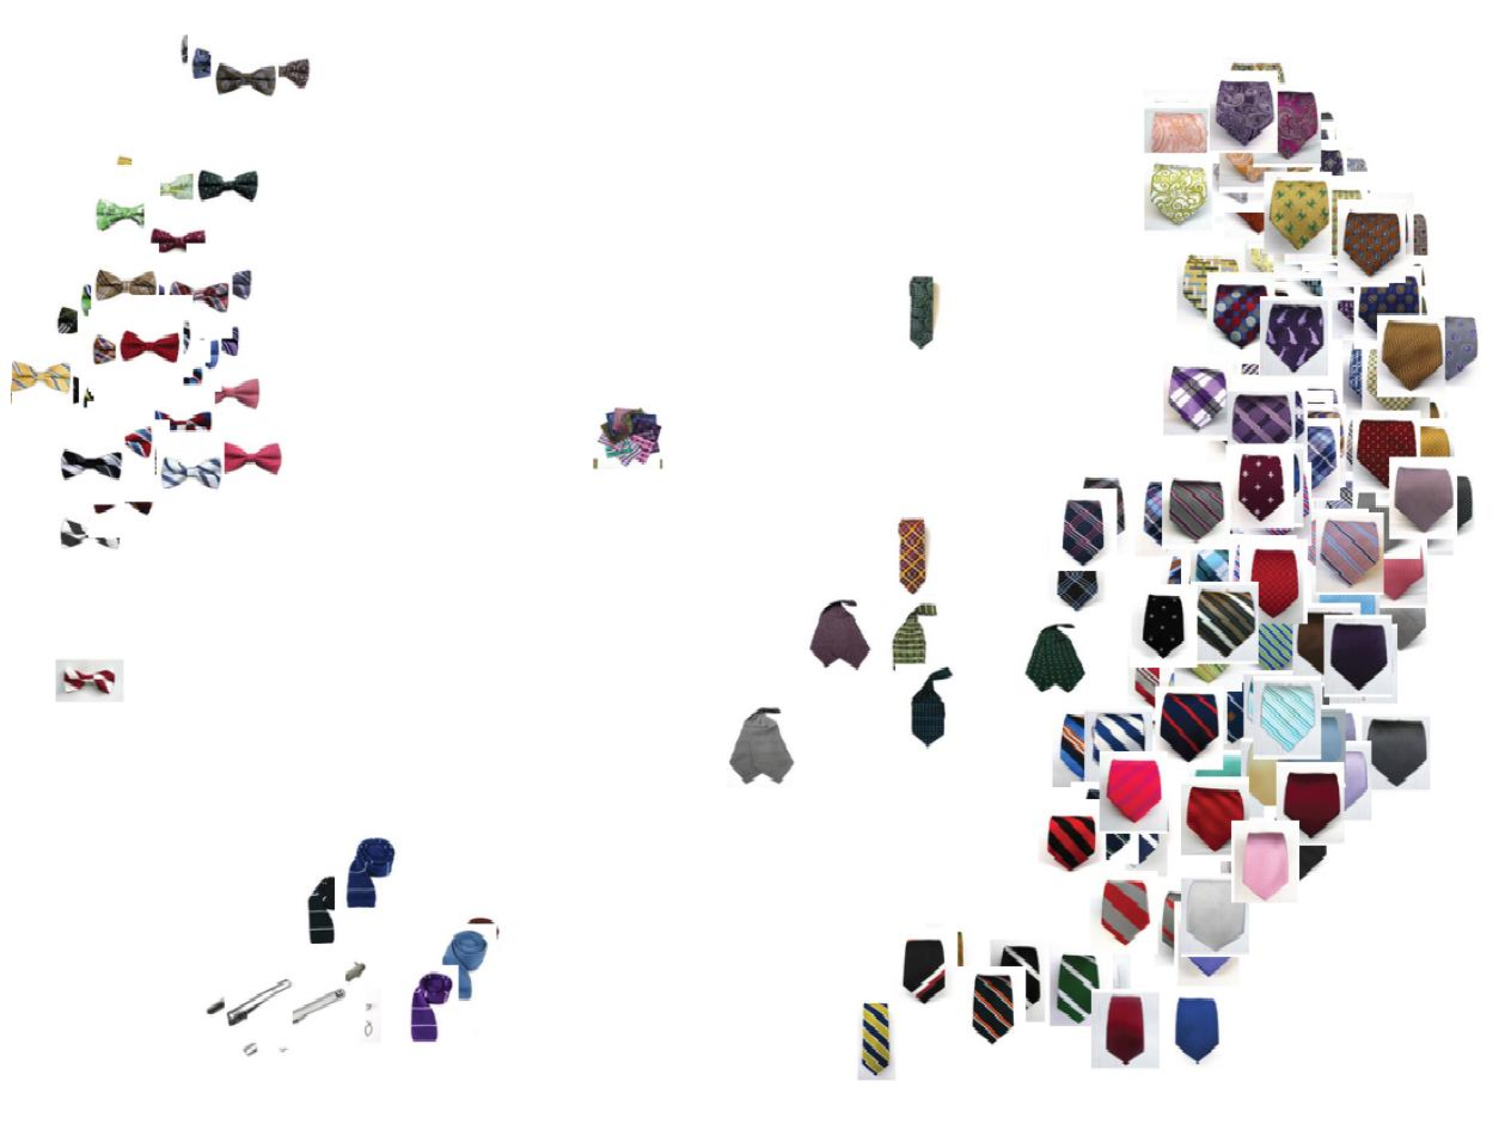
\includegraphics[width=3.5in]{neckties_pca2.pdf}}



\subsection{Optimization}


What we find here is that a low-rank constraint, which can be interpreted as fixing the dimensionality $d$ of $M \in \reals^{n \times d}$, is useful for generating high-quality questions to ask, but such a low-dimensional representation does not capture features of interest.  Fixing the diagonal to $S_{ii}=r$ gives a high-quality fit but does not generate quite as meaningful questions when we have little data.  Hence, when we have little data, we use the low-dimensional model in conjunction with our selection algorithm, for generating triples.  When we analyze the data which we have, we generally use the fixed-diagonal constraint without a rank bound.  Interestingly, the trace bound performed poorly in this setting.  In fact, a fixed-diagonal setting of $S_{ii}=r$ outperformed a trace bound of $nr$, even on training data.  This is counterintuitive because a fixed-diagonal setting of $S_{ii}=r$ directly implies a trace equal to $nr$.  The reason the optimization with the trace bound was failing is because the optimization problem is not convex, and hence gradient descent may reach local minima.  It seems that the trace bound and fixed-diagonal settings have different optimization landscapes, and the fixed-diagonal optimization performs better.



\section{System parameters and quality control}\label{sec:params}
We've described abstractly how our system is implemented.  This section describes parameters and specifics of our optimization algorithms and experiments.  Experiments were performed using the Mechanical Turk web service, where we define `Human Intelligence Tasks' to be performed by one or more users.  Each task consists of 50 comparisons and the interface is optimized to be performed with 50 mouse clicks (and no scrolling).  The mean completion time was approximately 2 minutes, for which workers were paid 15 cents.  This price was determined based upon worker feedback.  At 10 cents per task, though workers actively performed the tasks, some complained about low wages and several suggested that they be paid 15 cents per task.  At 15 cents per task, feedback was extremely positive -- the users reported that the tasks were enjoyable and requested more.  Initial experiments revealed a high percentage of seemingly random responses, but after closer inspection the vast majority of these poor results came from a small number of individuals.  To improve quality control, we imposed a limit on the maximum number of tasks a single user could perform on any one day, we selected users who had completed at least 48 tasks with a 95\% approval rate, and each task included 20\% triples for which there was tremendous agreement between users.  These ``gold standard'' triples were also automatically generated and proved to be an effective manner to recognize and significantly reduce cheating.  The system is implemented using Python, Matlab, and C, and runs completely automatically in Windows and Unix.

On each data set, for each object $a$ we first performed 10 triples comparing $a$ to random $b_i$ and $c_i$.  We then used the a low-dimensional fit (generally $d=3$ dimensions?) to the data to learn the relative model using a local optimization algorithm over $M \in \reals^{n\times d}$.  We used this model in order to generate triples.  We then generated about 20-30 additional adaptive triples for each object $a$.  For efficiency reasons, we generated five new triples each time, for each object in the database.

\subsubsection{Question phrasing and crowd alignment}
One interesting issue is how to frame similarity questions.  On the one hand, it seems purest in form to give the users carte blanche and ask only, ``is $a$ more similar to $b$ than $c$.''  On the other hand, in feedback users complained about these tasks and often asked what we meant by similarity.  Moreover, different users will inevitably weigh different features differently when performing comparisons.  For example, consider a comparisons of face images, where $a$ is a white male, $b$ is a black male, and $c$ is a white female.  Some users will consider gender more important in determining skin color, and others may feel the opposite is true.  Others may feel that the question is impossible to answer.  Consider phrasing the question as follows, ``At a {\em distance}, who would you be more likely to mistake for $a$: $b$ or $c$?''  For any two people, there is presumably some distance at which one might be mistaken for the other, so the question may seem more possible to answer for some people.  Second, users may more often agree that skin color is more important than gender, because both are easily identified close up by skin color may be identifiable even at a great distance.  While we haven't done experiments to determine the importance of question phrasing, anecdotal evidence suggests that users enjoy the tasks more when more specific definitions of similarity are given.

Two natural goals of question phrasing might be: (1) to align users in their ranking of the importance of different features and (2) to align user similarity  notions with the goals of the task at hand.  For example, if the task is to find a certain person, the question, ``which two people are most likely to be (genealogically) related to one another,'' may be poor because users may overlook features such as gender and age.  In our experiments on neckties, for example, the task was titled ``Which ties are most similar?'' and the complete instructions were:

\begin{quote}
Someone went shopping at a tie store and wanted to buy the item
on top, but it was not available. Click on item (a) or (b) below that would be the
{\bf best substitute}. Please repeat 50 times. We are researchers in Artificial Intelligence that are teaching computers what humans think similarity is on a bunch of things (letters, faces, fonts), so that we can build better programs.  (Please
don't answer randomly -- we have sophisticated ways of checking for that.) Thank
you!!
\end{quote}


\section{Algorithmic efficiency}\label{sec:efficient}

In this section, we describe an approach 


\section{Conclusion and Discussion}
In this work, we capture the crowd kernel using no machine attributes whatsoever.  Of course, when it is possible to well-approximate the crowd kernel automatically, that is desirable and our work could be used as a component of such a system. However, approximating it in general requires extremely good domain-specific features.  One of the biggest challenges in machine learning is selecting good features for a data sets.  Learning the crowd kernel without machine features, to some extent, sidesteps this issue.  This may be feasible at least for applications such as online stores where a small price per object may be reasonable.

For example, consider an online retailer that would like to perform data mining, say to learn how to better price jewelery from images. Features such as ``beauty'' or ``comfort'' may be evident to humans from images but would be hard to learn from current vision system.  An interesting direction for future research is to approximate the crowd kernel while forcing humans to articulate the features they are using in determining similarity.  

There is room to improve the adaptive component of our system.  First, one may make it online in the sense that it could add objects to the database one at a time or in batches, rather than having all the objects present up-front.  Second, it may be desirable to have personalized user-specific models as in \cite{??}, or group specific models.  For example, it may be interesting to contrast the Crowd Kernels of men and women on various domains.  Third, in the case where our model is not perfectly accurate, our algorithm suffers from the fact that the training distribution on queries is different from the test distribution.  Techniques such as importance weighting have been shown to be one practical solution to this problem for active learning \cite{BDL09}, and one might try to apply them to the problem at hand.

\bibliography{sim}
\bibliographystyle{icml2011}

\end{document}


% This document was modified from the file originally made available by
% Pat Langley and Andrea Danyluk for ICML-2K. This version was
% created by Lise Getoor and Tobias Scheffer, it was slightly modified
% from the 2010 version by Thorsten Joachims & Johannes Fuernkranz,
% slightly modified from the 2009 version by Kiri Wagstaff and
% Sam Roweis's 2008 version, which is slightly modified from
% Prasad Tadepalli's 2007 version which is a lightly
% changed version of the previous year's version by Andrew Moore,
% which was in turn edited from those of Kristian Kersting and
% Codrina Lauth. Alex Smola contributed to the algorithmic style files.


